\documentclass[12pt, letterpaper]{article}

% \usepackage{cmbright} % san serif font

% Chapters and sections config
\setcounter{secnumdepth}{5}
\setcounter{tocdepth}{5}
\makeatletter
\newcommand\subsubsubsection{\@startsection{paragraph}{4}{\z@}{-2.5ex\@plus -1ex \@minus -.25ex}{1.25ex \@plus .25ex}{\normalfont\normalsize\bfseries}}
\newcommand\subsubsubsubsection{\@startsection{subparagraph}{5}{\z@}{-2.5ex\@plus -1ex \@minus -.25ex}{1.25ex \@plus .25ex}{\normalfont\normalsize\bfseries}}
\makeatother

\usepackage{graphicx} % LaTeX package to import graphics
% \graphicspath{{images/}} % configuring the graphicx package

\parskip=5pt plus 1pt % adjusting space btw paragraphs, default 0pt plus 1pt
\parindent=15pt % indent in beginning of each paragraph, default 15pt

\title{My first \LaTeX{} document}
\author{Tung Le-Thanh\thanks{Funded by the Overleaf team.}}
\date{March 2023}

\begin{document}
\maketitle % create title from above preamble

\begin{abstract}
This is a simple paragraph at the beginning of the 
document. A brief introduction about the main subject.
\end{abstract}

\underline{Lorem ipsum} \textit{dolor sit} amet, 
\textbf{consectetur adipiscing elit}, % enter for good looking code, not affect pdf
\textit{sed do \emph{eiusmod} tempor}
\textbf{incididunt \emph{ut} labore} 
et dolore \emph{magna} aliqua. % double\multiple enter to new line

Ut ``enim'' ad % correct
"minim veniam", % not correct
quis ''nostrud'' exercitation ``ullamco`` % not correct, too
laboris nisi ut aliquip ex ea commodo consequat.

Egestas quis ipsum suspendisse ultrices gravida. \\ Habitasse platea dictumst vestibulum rhoncus est pellentesque elit. \newline Nibh venenatis cras sed felis eget velit aliquet. % newline, should not use
Turpis egestas sed tempus urna et. Est sit amet facilisis magna etiam tempor.

% add image
\begin{figure}[h]
    \centering
    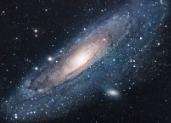
\includegraphics[width=0.3\textwidth]{images/universe.jpg}
    % \textwidth is horizontal length of paragraph
    \caption{A nice plot.}
    \label{fig:mesh1}
\end{figure}
As you can see in figure \ref{fig:mesh1}, the function grows near the origin. This example is on page \pageref{fig:mesh1}.

\newpage

% add item list (bullet)
\begin{enumerate}
  \item The individual entries are indicated with a black dot
  \item The text in the entries may be of any length.
    \begin{itemize}
      \item The individual entries are indicated with a black dot
      \item The text in the entries may be of any length.
    \end{itemize}
  \item The individual entries are indicated with a black dot
    \begin{enumerate}
      \item The individual entries are indicated with a black dot
      \item The text in the entries may be of any length.
    \end{enumerate}
\end{enumerate}

% math inline
\begin{math}
E=mc^2
\end{math} is typeset in a paragraph using inline math mode---as is $E=mc^2$, and so too is \(E=mc^2\).

% math mode
The mass-energy equivalence is described by the famous equation
\[ E=mc^2 \] discovered in 1905 by Albert Einstein. 

In natural units ($c = 1$), the formula expresses the identity
\begin{equation}
E=m
\end{equation}

% math symbol and equation
These can be combined and nested to write expressions such as
\[ T^{i_1 i_2 \dots i_p}_{j_1 j_2 \dots j_q} = T(x^{i_1},\dots,x^{i_p},e_{j_1},\dots,e_{j_q}) \]
 
We write integrals using $\int$ and fractions using $\frac{a}{b}$. Limits are placed on integrals using superscripts and subscripts:

\[ \int_0^1 \frac{dx}{e^x} =  \frac{e-1}{e} \]

Lower case Greek letters are written as $\omega$ $\delta$ etc. while upper case Greek letters are written as $\Omega$ $\Delta$.

Mathematical operators are prefixed with a backslash as $\sin(\beta)$, $\cos(\alpha)$, $\log(x)$ etc.

\newpage

\part{First part}
% \chapter{First chap} % only in book & report class
\section{First section}
This is the first section.
    \subsection{First subsection}
    This is the first subsection.
    \subsection{Second subsection}
        \subsubsection{Subsubsection}
            \paragraph{paragraph}
                \subparagraph{subparagraph}
            \paragraph{paragraph}
        \subsubsection{Subsubsection}
            \subsubsubsection{Subsubsubsection}
                \subsubsubsubsection{Subsubsubsubsection}
    
\section{Second section}
\section*{Unnumbered section}

% book class can be split into parts, chapters, sections, subsections,...

\newpage

\begin{center}
\begin{tabular}{c c c}
 cell1 & cell2 & cell3 \\ 
 cell4 & cell5 & cell6 \\  
 cell7 & cell8 & cell9    
\end{tabular}
\end{center}

\begin{center}
\begin{tabular}{|c|c|c|} 
 \hline
 cell1 & cell2 & cell3 \\ 
 \hline
 cell4 & cell5 & cell6 \\ 
 \hline
 cell7 & cell8 & cell9 \\ 
 \hline
\end{tabular}
\end{center}

\begin{center}
 \begin{tabular}{||c c c c||} 
 \hline
 Col1 & Col2 & Col2 & Col3 \\ [0.5ex] 
 \hline\hline
 1 & 6 & 87837 & 787 \\ 
 \hline
 2 & 7 & 78 & 5415 \\
 \hline
 3 & 545 & 778 & 7507 \\
 \hline
 4 & 545 & 18744 & 7560 \\
 \hline
 5 & 88 & 788 & 6344 \\ [1ex] 
 \hline
\end{tabular}
\end{center}

\newpage
  
\tableofcontents

\end{document}
